\documentclass[a4paper]{article}

\usepackage[margin=2cm]{geometry}
% Add the compsoc option for Computer Society conferences.
%
% If IEEEtran.cls has not been installed into the LaTeX system files,
% manually specify the path to it like:
% \documentclass[conference]{../sty/IEEEtran}

\usepackage{mathtools}
\usepackage{hyperref}
\usepackage{subfigure}
\usepackage[pdftex]{graphicx}
\graphicspath{{./fig/}}
\DeclareGraphicsExtensions{.pdf,.jpeg,.png}
\usepackage{todonotes}
\usepackage[nodayofweek]{datetime}

\newdateformat{dday}{
	\monthname[\THEMONTH], \THEYEAR
}


% Some very useful LaTeX packages include:
% (uncomment the ones you want to load)


% *** MISC UTILITY PACKAGES ***
%
%\usepackage{ifpdf}
% Heiko Oberdiek's ifpdf.sty is very useful if you need conditional
% compilation based on whether the output is pdf or dvi.
% usage:
% \ifpdf
%   % pdf code
% \else
%   % dvi code
% \fi
% The latest version of ifpdf.sty can be obtained from:
% http://www.ctan.org/tex-archive/macros/latex/contrib/oberdiek/
% Also, note that IEEEtran.cls V1.7 and later provides a builtin
% \ifCLASSINFOpdf conditional that works the same way.
% When switching from latex to pdflatex and vice-versa, the compiler may
% have to be run twice to clear warning/error messages.






% *** CITATION PACKAGES ***
%
%\usepackage{cite}
% cite.sty was written by Donald Arseneau
% V1.6 and later of IEEEtran pre-defines the format of the cite.sty package
% \cite{} output to follow that of IEEE. Loading the cite package will
% result in citation numbers being automatically sorted and properly
% "compressed/ranged". e.g., [1], [9], [2], [7], [5], [6] without using
% cite.sty will become [1], [2], [5]--[7], [9] using cite.sty. cite.sty's
% \cite will automatically add leading space, if needed. Use cite.sty's
% noadjust option (cite.sty V3.8 and later) if you want to turn this off.
% cite.sty is already installed on most LaTeX systems. Be sure and use
% version 4.0 (2003-05-27) and later if using hyperref.sty. cite.sty does
% not currently provide for hyperlinked citations.
% The latest version can be obtained at:
% http://www.ctan.org/tex-archive/macros/latex/contrib/cite/
% The documentation is contained in the cite.sty file itself.






% *** GRAPHICS RELATED PACKAGES ***
%


  % or other class option (dvipsone, dvipdf, if not using dvips). graphicx
  % will default to the driver specified in the system graphics.cfg if no
  % driver is specified.
  % \usepackage[dvips]{graphicx}
  % declare the path(s) where your graphic files are
  % \graphicspath{{../eps/}}
  % and their extensions so you won't have to specify these with
  % every instance of \includegraphics
  % \DeclareGraphicsExtensions{.eps}

% graphicx was written by David Carlisle and Sebastian Rahtz. It is
% required if you want graphics, photos, etc. graphicx.sty is already
% installed on most LaTeX systems. The latest version and documentation can
% be obtained at: 
% http://www.ctan.org/tex-archive/macros/latex/required/graphics/
% Another good source of documentation is "Using Imported Graphics in
% LaTeX2e" by Keith Reckdahl which can be found as epslatex.ps or
% epslatex.pdf at: http://www.ctan.org/tex-archive/info/
%
% latex, and pdflatex in dvi mode, support graphics in encapsulated
% postscript (.eps) format. pdflatex in pdf mode supports graphics
% in .pdf, .jpeg, .png and .mps (metapost) formats. Users should ensure
% that all non-photo figures use a vector format (.eps, .pdf, .mps) and
% not a bitmapped formats (.jpeg, .png). IEEE frowns on bitmapped formats
% which can result in "jaggedy"/blurry rendering of lines and letters as
% well as large increases in file sizes.
%
% You can find documentation about the pdfTeX application at:
% http://www.tug.org/applications/pdftex





% *** MATH PACKAGES ***
%
%\usepackage[cmex10]{amsmath}
% A popular package from the American Mathematical Society that provides
% many useful and powerful commands for dealing with mathematics. If using
% it, be sure to load this package with the cmex10 option to ensure that
% only type 1 fonts will utilized at all point sizes. Without this option,
% it is possible that some math symbols, particularly those within
% footnotes, will be rendered in bitmap form which will result in a
% document that can not be IEEE Xplore compliant!
%
% Also, note that the amsmath package sets \interdisplaylinepenalty to 10000
% thus preventing page breaks from occurring within multiline equations. Use:
%\interdisplaylinepenalty=2500
% after loading amsmath to restore such page breaks as IEEEtran.cls normally
% does. amsmath.sty is already installed on most LaTeX systems. The latest
% version and documentation can be obtained at:
% http://www.ctan.org/tex-archive/macros/latex/required/amslatex/math/





% *** SPECIALIZED LIST PACKAGES ***
%
%\usepackage{algorithmic}
% algorithmic.sty was written by Peter Williams and Rogerio Brito.
% This package provides an algorithmic environment fo describing algorithms.
% You can use the algorithmic environment in-text or within a figure
% environment to provide for a floating algorithm. Do NOT use the algorithm
% floating environment provided by algorithm.sty (by the same authors) or
% algorithm2e.sty (by Christophe Fiorio) as IEEE does not use dedicated
% algorithm float types and packages that provide these will not provide
% correct IEEE style captions. The latest version and documentation of
% algorithmic.sty can be obtained at:
% http://www.ctan.org/tex-archive/macros/latex/contrib/algorithms/
% There is also a support site at:
% http://algorithms.berlios.de/index.html
% Also of interest may be the (relatively newer and more customizable)
% algorithmicx.sty package by Szasz Janos:
% http://www.ctan.org/tex-archive/macros/latex/contrib/algorithmicx/




% *** ALIGNMENT PACKAGES ***
%
%\usepackage{array}
% Frank Mittelbach's and David Carlisle's array.sty patches and improves
% the standard LaTeX2e array and tabular environments to provide better
% appearance and additional user controls. As the default LaTeX2e table
% generation code is lacking to the point of almost being broken with
% respect to the quality of the end results, all users are strongly
% advised to use an enhanced (at the very least that provided by array.sty)
% set of table tools. array.sty is already installed on most systems. The
% latest version and documentation can be obtained at:
% http://www.ctan.org/tex-archive/macros/latex/required/tools/


%\usepackage{mdwmath}
%\usepackage{mdwtab}
% Also highly recommended is Mark Wooding's extremely powerful MDW tools,
% especially mdwmath.sty and mdwtab.sty which are used to format equations
% and tables, respectively. The MDWtools set is already installed on most
% LaTeX systems. The lastest version and documentation is available at:
% http://www.ctan.org/tex-archive/macros/latex/contrib/mdwtools/


% IEEEtran contains the IEEEeqnarray family of commands that can be used to
% generate multiline equations as well as matrices, tables, etc., of high
% quality.


%\usepackage{eqparbox}
% Also of notable interest is Scott Pakin's eqparbox package for creating
% (automatically sized) equal width boxes - aka "natural width parboxes".
% Available at:
% http://www.ctan.org/tex-archive/macros/latex/contrib/eqparbox/





% *** SUBFIGURE PACKAGES ***
%\usepackage[tight,footnotesize]{subfigure}
% subfigure.sty was written by Steven Douglas Cochran. This package makes it
% easy to put subfigures in your figures. e.g., "Figure 1a and 1b". For IEEE
% work, it is a good idea to load it with the tight package option to reduce
% the amount of white space around the subfigures. subfigure.sty is already
% installed on most LaTeX systems. The latest version and documentation can
% be obtained at:
% http://www.ctan.org/tex-archive/obsolete/macros/latex/contrib/subfigure/
% subfigure.sty has been superceeded by subfig.sty.



%\usepackage[caption=false]{caption}
%\usepackage[font=footnotesize]{subfig}
% subfig.sty, also written by Steven Douglas Cochran, is the modern
% replacement for subfigure.sty. However, subfig.sty requires and
% automatically loads Axel Sommerfeldt's caption.sty which will override
% IEEEtran.cls handling of captions and this will result in nonIEEE style
% figure/table captions. To prevent this problem, be sure and preload
% caption.sty with its "caption=false" package option. This is will preserve
% IEEEtran.cls handing of captions. Version 1.3 (2005/06/28) and later 
% (recommended due to many improvements over 1.2) of subfig.sty supports
% the caption=false option directly:
%\usepackage[caption=false,font=footnotesize]{subfig}
%
% The latest version and documentation can be obtained at:
% http://www.ctan.org/tex-archive/macros/latex/contrib/subfig/
% The latest version and documentation of caption.sty can be obtained at:
% http://www.ctan.org/tex-archive/macros/latex/contrib/caption/




% *** FLOAT PACKAGES ***
%
%\usepackage{fixltx2e}
% fixltx2e, the successor to the earlier fix2col.sty, was written by
% Frank Mittelbach and David Carlisle. This package corrects a few problems
% in the LaTeX2e kernel, the most notable of which is that in current
% LaTeX2e releases, the ordering of single and double column floats is not
% guaranteed to be preserved. Thus, an unpatched LaTeX2e can allow a
% single column figure to be placed prior to an earlier double column
% figure. The latest version and documentation can be found at:
% http://www.ctan.org/tex-archive/macros/latex/base/



%\usepackage{stfloats}
% stfloats.sty was written by Sigitas Tolusis. This package gives LaTeX2e
% the ability to do double column floats at the bottom of the page as well
% as the top. (e.g., "\begin{figure*}[!b]" is not normally possible in
% LaTeX2e). It also provides a command:
%\fnbelowfloat
% to enable the placement of footnotes below bottom floats (the standard
% LaTeX2e kernel puts them above bottom floats). This is an invasive package
% which rewrites many portions of the LaTeX2e float routines. It may not work
% with other packages that modify the LaTeX2e float routines. The latest
% version and documentation can be obtained at:
% http://www.ctan.org/tex-archive/macros/latex/contrib/sttools/
% Documentation is contained in the stfloats.sty comments as well as in the
% presfull.pdf file. Do not use the stfloats baselinefloat ability as IEEE
% does not allow \baselineskip to stretch. Authors submitting work to the
% IEEE should note that IEEE rarely uses double column equations and
% that authors should try to avoid such use. Do not be tempted to use the
% cuted.sty or midfloat.sty packages (also by Sigitas Tolusis) as IEEE does
% not format its papers in such ways.





% *** PDF, URL AND HYPERLINK PACKAGES ***
%
%\usepackage{url}
% url.sty was written by Donald Arseneau. It provides better support for
% handling and breaking URLs. url.sty is already installed on most LaTeX
% systems. The latest version can be obtained at:
% http://www.ctan.org/tex-archive/macros/latex/contrib/misc/
% Read the url.sty source comments for usage information. Basically,
% \url{my_url_here}.



\usepackage[toc,page]{appendix}
\usepackage{color}
%MACROS---
\newcommand{\reffig}[1]{Fig. \ref{#1}}
\newcommand\xput[2][0.5]{%
    \rule{#1\linewidth}{0pt}\makebox[0pt][c]{#2}\hfill}

\title{Report on Lab 1 \& Lab 2 in EDA282, Parallel Computer Organization and Design}
\date{October 2014}
\author{Dan Larsson, Jonas Hemlin
\\Master Program of Embedded Electronic Systems Design\\
Chalmers University of Technology, Gothenburg, Sweden\\
Email: \{larsdan, jhemlin\}@student.chalmers.se}


\definecolor{mygreen}{rgb}{0,0.6,0}
\definecolor{mygray}{rgb}{0.1,0.1,0.1}
\definecolor{mymauve}{rgb}{0.58,0,0.82}

\lstset{ 
	language=C,
	backgroundcolor=\color{white},
	basicstyle=\small,        % the size of the fonts that are used for the code
	breakatwhitespace=false,         % sets if automatic breaks should only happen at whitespace
	breaklines=true,                 % sets automatic line breaking
	captionpos=t,                    % sets the caption-position to bottom
	commentstyle=\color{mygreen},    % comment style
	deletekeywords={},
	morekeywords={pragma,schedule,reduction,omp,single,private,shared, parallel},            
	extendedchars=true,              % lets you use non-ASCII characters; for 8-bits encodings only, does not work with UTF-8
	frame=single,                    % adds a frame around the code
	keepspaces=true,                 % keeps spaces in text, useful for keeping indentation of code (possibly needs columns=flexible)
	keywordstyle=\color{blue},       % keyword style
	numbers=left,                    % where to put the line-numbers; possible values are (none, left, right)
	numbersep=8pt,                   % how far the line-numbers are from the code
	numberstyle=\footnotesize\color{mygray}, % the style that is used for the line-numbers
	rulecolor=\color{black},         % if not set, the frame-color may be changed on line-breaks within not-black text (e.g. comments (green here))
	showspaces=false,                % show spaces everywhere adding particular underscores; it overrides 'showstringspaces'
	showstringspaces=false,          % underline spaces within strings only
	showtabs=false,                  % show tabs within strings adding particular underscores
	stepnumber=2,                    % the step between two line-numbers. If it's 1, each line will be numbered
	stringstyle=\color{mymauve},     % string literal style
	tabsize=2                       % sets default tabsize to 2 spaces                   % show the filename of files included with \lstinputlisting; also try caption instead of title
}




\begin{document}
\maketitle
$$ Cost = 1 * (WriteHit+ReadHit) + 30 * (readMissesServicedByShared + invalidationsSent)$$ $$+ 20 * LLCHit + 50 * LLCMiss $$
\section{Introduction}
\label{sec:int}
These laboratory assignments aim to increase our knowledge of different cache coherence protocols. To reach this goal, we simulate cache coherence protocols (CCP) on a modeled cache coherent multi-core system using diverse benchmarks. Three cache coherence protocols are targeted; MSI, MESI, and MESI-MG, where the last protocol is an modified version of MESI optimized for migratory sharing. The system model have a shared Last Level Cache (LLC), and each processor have a private L1 cache. Snooping based write-invalidate cache coherence protocols are used by the private L1 caches to ensure coherence, and a simple bus stand for the communication between LLC and private caches. The system is modeled by the Pin tool MultiCacheSim and Pin. In listing~\ref{lst:setup} is the command used for simulating a CCP on the modeled system with a chosen benchmark. To relate the simulation results to excecution time, Eq. \ref{eq:cycles} is used. 



\begin{lstlisting}[label=lst:setup, basicstyle=\scriptsize, caption={Command used for simulation.}]
#> ./pin -mt -t ./source/tools/MultiCacheSim/obj-intel64/mcs.so -csize 65536 -bsize 64 -assoc 8 -llc -llcsize 4194304 -llcbsize 64 -llcassoc 16 -numcaches 8 -protos ./source/tools/MultiCacheSim/obj-intel64/mcs_<CCP>.so -- <benchmark> [#threads,..]
\end{lstlisting}
\begin{equation}
	$$\label{eq:cycles}$$
	Cycles = 1 * (WriteHit+ReadHit) + 30 * (readMissesServicedByModified + invalidationsSent)$$ $$+ 20 * LLCHit + 50 * LLCMiss
\end{equation}
\section{Lab 1}
\label{sec:lab1}
\section{Lab 2}
\label{sec:lab2}
For the second part of the lab the task is to parallelize a serial implementation of the Red-Back Gauss-Seidal algorithm. This is done using OpenMP (Open \textbf Multi-\textbf Processing) which is an API for forming multi-threaded programs in C, C++, and Fortran. This parallel version is evaluated using the same simulator and CCPs as in \nameref{sec:lab1}. 

\subsection{Task 1}
The program reads a matrix on the form $n \times n$ containing data points from a file. To make the program simpler and avoid special cases a padding is added to the matrix changing its dimensions to $(n+2) \times (n+2)$. Then every other data point, here by called red dots, is looped through. For every red dot an average of itself and its neighbors to the west, south, north, and east is calculated and written as the dots new value. For all the other data points, called black dots, the same thing is performed. The difference of the dots new and old value is added together and the process is repeated until this accumulated difference of averages, divided by $n^2$, is smaller than $0.01$. After the program finishes its execution the matrix have converged to an average of all red and black dots.

The distribution of the red and black dots forms a chess pattern. This means that when we calculate the average for a dot and its neighbors, all the neighbors are of the other color. As such, when going through for example the red dots there is no need to invalidate any other dots because the black dots are only read and you are the only one accessing your red dot.

\subsection{Task 2}
\label{subsec:lab2:task2}
In listing~\ref{lst:solve} a parallelized version of the function \texttt{void Solve(double **A)} are shown. The parallelization have been done using directives from the OpenMP API. Only this function is shown as the other parts of the program for reading the input file and printing to the console is not included in the performance analysis. The approach taken for making the function execute in parallel is to distribute the lines of the matrix evenly between all threads. This is done twice, once for the red dots and once for the black. Only one thread resets \texttt{diff} to zero on line 5 and test whether the program is finished or not on line 25. At each for loop that goes through the red and black dots the directive \texttt{reduction(+:diff)} is used which causes each thread to have its own private version of \texttt{diff} that all gets added together after the for loop.

\subsection{Task 3}
To be able to evaluate the program described in \nameref{subsec:lab2:task2} we decide to mimic the working set sizes in \nameref{sec:lab1}. However, the provided data files does not include a matrix big enough to fill neither each threads L1 cache or the LLC cache.

In \reffig{fig:lab2} results from running the parallelized version of the program in the simulator with different CCPs and different matrix dimensions are shown. It can be seen that using MESI over MSI does not cause any noticeable boost in performance. This is because the gain of the extra E state becomes of no importance as the cache lines is in the M state most of the time. Some benefit of the E state can though be seen in Table~\ref{tbl:lab2} as the amount of \textit{WriteMisses} and \textit{InvalidationsSent} are a bit lower for MESI than MSI and the gap becomes bigger as the matrix size increases. This does not show in \reffig{fig:lab2} as the cycle count are not dominated by \textit{WriteMisses} and \textit{InvalidationsSent}.

Changing to MESI-MG yields a huge performance degradation of 420\%, 394\%, and 430\% for matrix size 25, 100, and 200 respectively. This comes from the sharing performed of the brim lines between threads. For each read of a dot in any of these lines, the dot gets migrated over to the thread performing the read. This frequent migration of dots generates a large amount of \textit{ReadMissesSerivcedByModfied} as can be seen in Table~\ref{tbl:lab2}. The overhead stays fairly constant compared to the other CCPs when the matrix size increases. This is duo to the proportion of sharing between the threads stays the same.  

\begin{figure}[t]
	\center
	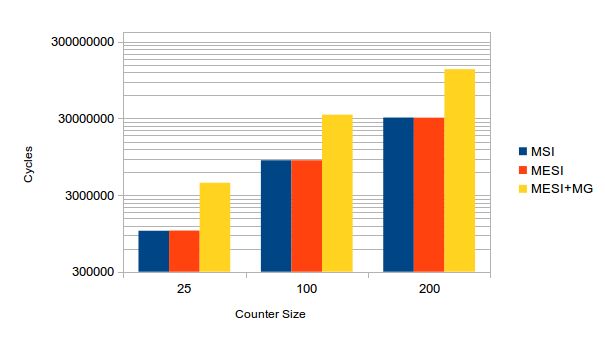
\includegraphics[width=0.8\textwidth]{lab2bars}
	\caption{Results from simulation of the parallelized benchmark for all cache coherence protocols combined with different working sets.}
	\label{fig:lab2}
\end{figure}

\subsection{Task 4}
%\todo[inline]{Outline a strategy to modify the MESI protocol to support the O state. Analyze the MESI\_SMPCache.cpp source to understand how the MESI protocol is currently modeled. Discuss changes that need to be made to the readLine, writeLine, readRemoteAction, and writeRemoteAction functions. Show the necessary changes in pseducode. Should the code that tracks cache access statistics be modified? If so, how?}

To add the Owner (O) state to the existing MESI CCP only some small changes are needed. In \textit{readLine()} and \textit{remoteWriteAction()} no changes are needed. Turning to \textit{readRemoteAction()}, transitions from the E, M, and O states to the O state are added, and all of these transitions provide data to the calling cache. The action taken when in the shared state is removed. For the \textit{writeLine()} the only change needed is to take the same actions when in the O state as in the S state. For the cache access statistics there is no need to change anything

\par\noindent
\begin{minipage}[t]{.5\textwidth}
\begin{lstlisting}[language=C,frame=lrtb]
In readLine()
	if(MODIFIED) {...}
	if(EXCLUSIVE) {...}

	if(SHARED)
		return data		

In writeRemoteAction()
	if(SHARED) {...}
\end{lstlisting}%
\end{minipage}%
\hfill
\begin{minipage}[t]{.5\textwidth}
\begin{lstlisting}[frame=lrtb]
In readLine()
	if(MODIFIED || EXCLUSIVE || OWNER) 
		state = OWNER
		return data

	if(SHARED)
	{}

In writeRemoteAction()
	if(SHARED || OWNER) {...}
\end{lstlisting}%
\end{minipage}%

\section{Discussion} 
\label{sec:disc}

% \begin{table*}[t]
% 	\caption{\label{tbl:summary}Summarized stuff.}
%         \begin{center}
% 			\normalsize
% 			\begin{tabular}{ l r r r r r r}
% 				\textbf{Technique} & \parbox{2cm}{ \textbf{Refresh \linebreak information}} & \textbf{Modifies} & \parbox{1.7cm}{ \textbf{Refresh \linebreak reduction}} & \parbox{2.2cm}{ \textbf{DRAM power \linebreak reduction}} & \parbox{1.2cm}{\textbf{Storage \newline Overhead}} & \parbox{1.5cm}{\textbf{Performance impact}} \vspace{0.05cm} \\
% 				\hline
% 				\textit{Smart Refresh} & A & MC & 59\% & $12.13\%$ & $0.0048\%$  & Unknown  \\
% 				\textit{Refrint} & A & MC, (?) & N/A & N/A  & $0.005\%$  & N/A  \\
% 				\hline
% 				\textit{RAIDR} & R & MC & $74.6\%$ & $8.3\%$  & $0.031\%$  & $4.1\%$  \\
% 				\textit{DTail-R} & R & MC, DDRx & $87.9\%$ & $\approx 23\%$  & $0.0045\%$ & $\approx$ \textit{RAIDR} \\
% 				\textit{RIO} & R & OS & $87.5\%$ & Unknown  & $0.1\%$  & $4.5\%$ \\
% 				\textit{SECRET} & R & MC & $87.5\%$ & $18.6\%$  & $\approx 0.01\%$  & $\pm 1.4\%$  \\
% 				\hline
% 				\textit{DTail-V} & V & MC, DDRx, (OS) & $\approx 10\% \to 90\% $ & $41.7\%$ \textit{PARIS}  & $0.0015\%$ & $4.4\%$ \textit{PARIS}  \\
% 				\textit{PARIS} & V & MC, OS & $\approx 10\% \to 90\%$ & Unknown  & $0.0015\%$  & Unknown \\
% 				\hline
% 				\textit{Flikker} & T & MC, OS, Apps & Unknown & $20\% \to 25\%$  & $0.005\%$  & $-1\%$   \\
% 				\textit{Sparkk} & V, T  & MC, OS, Apps &  $50\%$ \textit{Flikker} & Unknown & Unknown  & Unknown \\
% 				\hline
% 			\end{tabular}
% 		\end{center}
% \end{table*}
In the following section we compare all surveyed techniques more thoroughly and present some of our thoughts on their future potential.

\subsection{Advantages and disadvantages of each approach}
First of, we believe that the footprint of each surveyed technique is negligible when DRAM capacity increases. This as no technique has a larger storage overhead than $0.1\%$ of DRAM capacity.

%\subsubsection*{Access Recency} 
Access Recency techniques becomes less effective when DRAM capacity scales, as it is probable that the access rate per row will decrease. Among the approaches, this is one of the easier to implement, as it essentially only needs to track DRAM accesses and count the time between them. Techniques based on the other approaches can achieve the same or better results even when the access rate is low.

%\subsubsection*{Retention Time}
Using R as the refresh data gives a high efficiency independent of DRAM capacity, running applications, and memory utilization. A downside is that retention time profiling of the DRAM has to be performed in conjunction with first system startup. As retention time is highly dependent on temperature variations and has to be accounted for, which some techniques do; RAIDR, and RIO. 

%\subsubsection*{Validity} 
The V approach scales well, as it is more probably that more rows becomes invalid when DRAM capacity increases. It also produce high efficiency in many common systems. However, support on a OS level is needed to gather the V data, which increases the complexity. 

%\subsubsection*{Data Tolerance} 
The efficiency of T based techniques is dependent of memory utilization besides of data with low criticality, as T do not target invalid memory areas. Using T information can yield a high decrease of refresh operations, but heavy modifications in several layers are required. 

\subsection{Modifications required and future potential}

%\todo[inline]{describe the table}
%-no area info

The method used for refresh can affect the possibility of a technique to scale. Techniques that relies on ROR can have problems with large DRAM capacities. This as the number of rows will be to large for ROR to refresh within the maximum refresh period. One example of this is PARIS, which fails to work on a system with \textit{32~GB} of memory \cite{dtail}. 

Techniques which only require OS modifications is easier to adopt than those who need other changes. RIO is a good example of a technique which can be adopted after light kernel updates. The potential of RIO is significant compared to the modifications needed, as it reduces refreshes to the same degree as R based techniques that need hardware modifications at the cost of higher storage overhead. Moreover, all other surveyed techniques require specific support from at least the MC.

Among the techniques which modifies the MC, there are one group that in addition to their logic also have large tables in the MC; Smart Refresh, Refrint, RAIDR, and PARIS. Another group stores it's data in the DRAM instead of the MC; SECRET, and DTail. The advantage of keeping the refresh data in DRAM is lower MC area overhead and cheaper memory, whereas the downside is that the data has to be cached or prefetched to the MC to mitigate the longer access time of DRAM. DTail has additional need of a extension to the DDRx standard, which can complicate the adoption of the technique.

The techniques that requires the heavies modifications are those based on T. Even so, their potential is good and Sparkk's total DRAM power reduction is high, but the changes needed will not be transparent for the application programmer, who has to learn the concept of approximate data in order for the technique to be efficient. This is maybe to much to ask, therefor we do believe that T based techniques has lower future potential than R and V based techniques.

We believe that the R and V approaches is the most promising for the future. This as techniques based on A, even though they are quite simple to implement, the trend is to increase the DRAM capacity and cache structures, which speaks against the usage of this approach. But of course, in systems that does not follow these trends, Access Recency can have a chance to be adopted. Such systems could for example be small embedded systems or large shared memory systems with small or no cache and many cores. 

3D stacked DRAM will affect all approaches. The higher temperature increases the refresh rate and stretches the demands for techniques using ROR to lower the refresh rate in order to keep up. The temperature will also be more uneven across the device due to the stacking, which give higher requirements for tracking the variations and adapt to them. One technique not surveyed in this paper, proposed by Sadri et al. \cite{tempaware}, tracks the temperature in different regions of a 3D DRAM and adapts the refresh rate accordingly in these areas.

\subsection{Combining techniques}

To achieve a larger DRAM power reduction, techniques from different approaches can be combined. An example of this is RIO+PARIS, which increases the refresh reduction to $93.8\%$. If DTail-RV is used instead, the refresh reduction increases to $98.9\%$. DTail could be extended with an arbitrary T data acquisition technique for further improvements. All surveyed techniques target to reduce refresh power, but to achieve the greater goal of minimizing total DRAM power, smart scheduling of all DRAM accesses could advantageously be incorporated. 

For example has Isen and John proposed the smart scheduling technique ESKIMO \cite{eskimo}, which focus at reducing total DRAM power through optimizing the accesses to the DRAM. By using one bit of a cache row to denote whether it hold nonsense data, it becomes possible to resolve some memory accesses in the caches, which otherwise would have needed to access DRAM. A memory region is regarded as nonsense if it has been deallocated, or allocated but not written to. The ISA has to be extended to provide the allocation and deallocation information. If a block has to be replaced in a write-through cache and the replaced block is dirty but also deallocated, the cache can ignore writing the replaced block to memory. Similarly, a write miss to a newly allocated area results in a read access that can also be ignored. Combining ESKIMO with the selective refresh implementation proposed by Ohsawa \cite{ohsawa}, $39\%$ of total DRAM power was saved on average.


\newpage
\begin{appendices}
\section{Parallelized program for Lab 2}
\centerline{
\begin{minipage}{1.0\textwidth}
\lstinputlisting[caption={\textit{Parallel version of original} \texttt{void Solve(double **A).}}, label={lst:solve}]{include/solve.c}
\end{minipage}
}
\end{appendices}
\end{document}